%% ============================================================
%%  FIN1 – Personal Financial Planning Report
%%  Compiler : XeLaTeX  (Overleaf: Menu → Compiler → XeLaTeX)
%%  Format   : Executive Corporate Finance Template
%%  Reference: APA 7th Edition
%% ============================================================
\documentclass[12pt,a4paper]{report}

%% ── FONT CONFIGURATION (Executive Corporate Style) ──────────
\usepackage{fontspec}
\setmainfont{Cambria}
\newfontfamily\headingfont{Calibri}[BoldFont={Calibri Bold}, ItalicFont={Calibri Italic}]

%% ── PAGE GEOMETRY (Symmetric Corporate Standard) ──────────
\usepackage[
  left   = 2.5cm,
  right  = 2.5cm,
  top    = 2.5cm,
  bottom = 2.5cm,
  includeheadfoot
]{geometry}

%% ── LINE SPACING & PARAGRAPH ────────────────────────────────
\usepackage{setspace}
\onehalfspacing
\setlength{\parindent}{1.27cm}
\setlength{\parskip}{6pt}

%% ── COLORS (McKinsey / BCG Style Corporate Theme) ──────────
\usepackage[table]{xcolor}
\definecolor{corpnavy}{HTML}{002D62}  % McKinsey/Deloitte style Navy
\definecolor{corpblue}{HTML}{0078D4}  % Accent Blue
\definecolor{corpgray}{HTML}{5E5E5E}  % Neutral gray for running elements
\definecolor{corplight}{HTML}{F4F6F9} % Light background for rows and boxes
\definecolor{corpborder}{HTML}{D1D5DB}% Border gray
\definecolor{corpcharcoal}{HTML}{2D3748}% Soft charcoal for body text (more premium than pure black)

\AtBeginDocument{%
  \color{corpcharcoal}%
  \arrayrulecolor{corpnavy}%
}

%% ── TABLES & FIGURES ────────────────────────────────────────
\usepackage{graphicx}
\usepackage{wrapfig}             % figure beside text
\usepackage{booktabs}
\usepackage{longtable}
\usepackage{float}               % [H] forced placement
\usepackage{array}
\usepackage{tabularx}            % auto-width columns
\newcolumntype{L}{>{\raggedright\arraybackslash}X}  % left-aligned auto-width
\usepackage{makecell}

%% ── MATH ────────────────────────────────────────────────────
\usepackage{amsmath}
\usepackage{unicode-math}     % XeLaTeX math font support
\usepackage{xurl}             % allow URL breaks at any character

%% ── CAPTION FORMAT (APA 7th Edition) ────────────────────────
\usepackage{caption}
\DeclareCaptionFormat{apatable}{%
  \textbf{#1#2}\\[3pt]\textit{#3}%
}
\captionsetup[table]{
  format          = apatable,
  labelsep        = none,
  justification   = raggedright,
  singlelinecheck = false,
  position        = top,
  skip            = 4pt
}
\captionsetup[figure]{
  labelfont       = it,
  textfont        = it,
  labelsep        = period,
  justification   = raggedright,
  singlelinecheck = false,
  position        = below,
  skip            = 8pt
}

%% ── HEADER / FOOTER ─────────────────────────────────────────
\usepackage{fancyhdr}
\pagestyle{fancy}
\fancyhf{}
\fancyhead[L]{\fontsize{9}{11}\selectfont\headingfont\color{corpgray}FIN1 --- Personal Financial Planning Report}
\fancyhead[R]{\fontsize{9}{11}\selectfont\headingfont\color{corpgray}\leftmark}
\fancyfoot[R]{\fontsize{10}{12}\selectfont\headingfont\color{corpnavy}\thepage}
\renewcommand{\headrulewidth}{0.5pt}
\renewcommand{\footrulewidth}{0pt}
\addtolength{\headheight}{2.5pt}
\renewcommand{\headrule}{\hbox to\headwidth{\color{corpborder}\leaders\hrule height \headrulewidth\hfill}}

\fancypagestyle{plain}{%
  \fancyhf{}%
  \fancyfoot[R]{\fontsize{10}{12}\selectfont\headingfont\color{corpnavy}\thepage}%
  \renewcommand{\headrulewidth}{0pt}%
}

%% ── CHAPTER & SECTION HEADINGS (titlesec) ───────────────────
\usepackage{titlesec}

%% CHAPTER: "PHASE N" centred 18pt bold Calibri, chapter title below
\titleformat{\chapter}[display]
  {\headingfont\fontsize{18}{22}\selectfont\bfseries\color{corpnavy}\centering}
  {\MakeUppercase{\chaptertitlename}\ \color{corpblue}\thechapter}
  {8pt}
  {\headingfont\fontsize{18}{22}\selectfont\bfseries\centering}
\titlespacing*{\chapter}{0pt}{0pt}{30pt}

%% SECTION: 14pt bold Calibri, with thick blue accent line below
\titleformat{\section}
  {\headingfont\fontsize{14}{17}\selectfont\bfseries\color{corpnavy}}
  {\color{corpblue}\thesection}
  {1em}{}
  [\vspace{3pt}{\color{corpblue}\hrule height 1.5pt}]
\titlespacing*{\section}{0pt}{16pt}{8pt}

%% SUBSECTION: 12pt bold italic Calibri
\titleformat{\subsection}
  {\headingfont\fontsize{12}{15}\selectfont\bfseries\itshape\color{corpnavy}}
  {\color{corpblue}\thesubsection}
  {1em}{}
\titlespacing*{\subsection}{0pt}{12pt}{6pt}

%% ── TABLE OF CONTENTS ───────────────────────────────────────
\usepackage{tocloft}
\renewcommand{\cftchapfont}{\headingfont\bfseries\color{corpnavy}}
\renewcommand{\cftchappagefont}{\headingfont\bfseries\color{corpnavy}}
\renewcommand{\cftsecfont}{\headingfont\color{corpcharcoal}}
\renewcommand{\cftsecpagefont}{\headingfont\color{corpcharcoal}}
\setlength{\cftbeforechapskip}{4pt}
\renewcommand{\cftchapleader}{\cftdotfill{\cftdotsep}}

%% ── LISTING STYLES (enumitem) ────────────────────────────────
\usepackage{enumitem}
\setlist[itemize,1]{label=\color{corpblue}\textbullet}
\setlist[itemize,2]{label=\color{corpblue}\normalfont\bfseries --}

%% ── TAKEAWAY BOXES (tcolorbox) ──────────────────────────────
\usepackage[most]{tcolorbox}
\newtcolorbox{takeawaybox}[1][]{
  colback=corplight,
  colframe=corpnavy,
  arc=4pt,
  outer arc=4pt,
  boxrule=0.5pt,
  leftrule=4pt,
  top=10pt,
  bottom=10pt,
  left=14pt,
  right=14pt,
  fonttitle=\headingfont\bfseries\color{white},
  fontupper=\normalfont,
  sharp corners=northeast,
  #1
}

%% ── APA REFERENCES: hanging indent ─────────────────────────
\usepackage{hanging}

%% ── HYPERLINKS ──────────────────────────────────────────────
\usepackage{hyperref}
\hypersetup{
  colorlinks = true,
  linkcolor  = corpnavy,
  citecolor  = corpnavy,
  urlcolor   = corpblue,
  pdfauthor  = {Vu Duc Huy},
  pdftitle   = {FIN1 - Personal Financial Planning Report},
}

%% ── CHAPTER PREFIX: "Phase" → displayed as "PHASE N" ───────
\renewcommand{\chaptername}{Phase}

% ─────────────────────────────────────────────────────────────
\begin{document}

\begin{titlepage}
\centering
\color{corpnavy}

\vspace*{1cm}
{\headingfont\bfseries\Large FOREIGN TRADE UNIVERSITY}\\[4pt]
{\headingfont\bfseries\Large FACULTY OF BANKING AND FINANCE}\\[10pt]
{\color{corpblue}\hrule height 2pt}\\[2cm]


\includegraphics[width=5cm]{figures/ftu_logo.png}\\[2cm]

{\headingfont\fontsize{22}{28}\selectfont\bfseries PERSONAL FINANCIAL PLANNING REPORT}\\[0.5cm]
{\headingfont\fontsize{14}{18}\selectfont\color{corpblue} Internship \& Career Finance Roadmap}\\[1.5cm]

{\headingfont\large\bfseries Course: FIN 1 --- Financial Planning}\\[4pt]
{\headingfont\large Class: TCHE322(2526-2)GD2.02}\\[3cm]

\begin{tabular}{@{}ll@{}}
  {\headingfont\bfseries Submitted to:} & {\headingfont MSc. Nghiêm Anh Thư} \\[8pt]
  {\headingfont\bfseries Prepared by:}  & {\headingfont Vũ Đức Huy} \\[8pt]
  {\headingfont\bfseries Student ID:}   & {\headingfont 2412340057} \\[8pt]
  {\headingfont\bfseries Major:}        & {\headingfont K63 -- Anh 01 -- BIF.H (Banking \& Finance)} \\
\end{tabular}

\vfill
{\headingfont\bfseries Hanoi, June 2026}

\end{titlepage}

\clearpage

\rowcolors{2}{corplight}{white}

{\singlespacing\tableofcontents}
\clearpage

%% Introduction (unnumbered — no "Phase" prefix)
\chapter*{Introduction to Personal Financial Planning}
\addcontentsline{toc}{chapter}{Introduction to Personal Financial Planning}

Second year of university is a strange time to be thinking about retirement. But that is roughly where this report starts---with the question of what someone at 20 needs to do today to have a comfortable life at 60, and what the 40 years in between should look like. The gap between now and then is large enough that it is easy to ignore. It is also exactly long enough that the decisions made in it compound into something either very good or very hard to undo.

This report is a personal financial plan for me, Vũ Đức Huy, a second-year Banking and Finance student at Foreign Trade University, Hanoi. I live in a family-owned 72~m\textsuperscript{2} apartment where rent, electricity, and water are covered by my family, which keeps my cost of living much lower than most students in Hanoi. My income runs from three sources at the same time: a 3,000,000~VND internship allowance from kNowHow Consultant, average freelance software income of 2,500,000~VND, and a 4,000,000~VND monthly family allowance---9,500,000~VND total. Two people shape how I think about discipline and preparation: Max Verstappen (Formula~1) and Chou Tien Chen (Badminton). Not for their results, but for how they work.

The report covers ten phases: spending analysis, goal-setting, personal financial statements, income tax, budgeting, credit strategy, vehicle purchase, stock investment, insurance, and retirement planning. All numbers come from a real 30-day transaction log (May~7 to June~4, 2026) exported from my ABBank app. The path traced runs from 9,500,000 VND per month now to a projected 300,000,000 VND per month as a BCG Partner or technology founder, with a retirement target at age~60.


%% Phases 1–10 (auto-numbered PHASE 1 … PHASE 10)
\chapter{Analysis of 30-Day Spending and Consumption Patterns}

I tracked every personal transaction from May~7 to June~4, 2026---67 transactions exported from my ABBank app. Major household costs (apartment fees, electricity, water) are paid by my family and excluded. The data covers only the spending I personally control.

\section{Spending Summary by Category}

\begin{table}[h!]
\caption{30-Day Personal Spending Breakdown}
\label{tab:spending_breakdown}
\begin{tabularx}{\linewidth}{@{}lrrL@{}}
\toprule
\textbf{Category} & \textbf{Total (VND)} & \textbf{Share (\%)} & \textbf{Key Drivers} \\
\midrule
Food            & 3,810,866 & 73.4\% & Dining out, social gatherings, groceries \\
Sports          &   759,000 & 14.6\% & Badminton court bookings, racket restringing \\
Shopping online &   474,999 &  9.2\% & Phone cards, e-commerce purchases \\
Entertainment   &   145,000 &  2.8\% & Gaming cafes, digital subscriptions \\
\midrule
\textbf{Total}  & \textbf{5,189,865} & \textbf{100.0\%} & \\
\bottomrule
\end{tabularx}
\end{table}

\section{Consumption Pattern Analysis}

\begin{wrapfigure}{r}{0.42\textwidth}
  \vspace{-10pt}
  \centering
  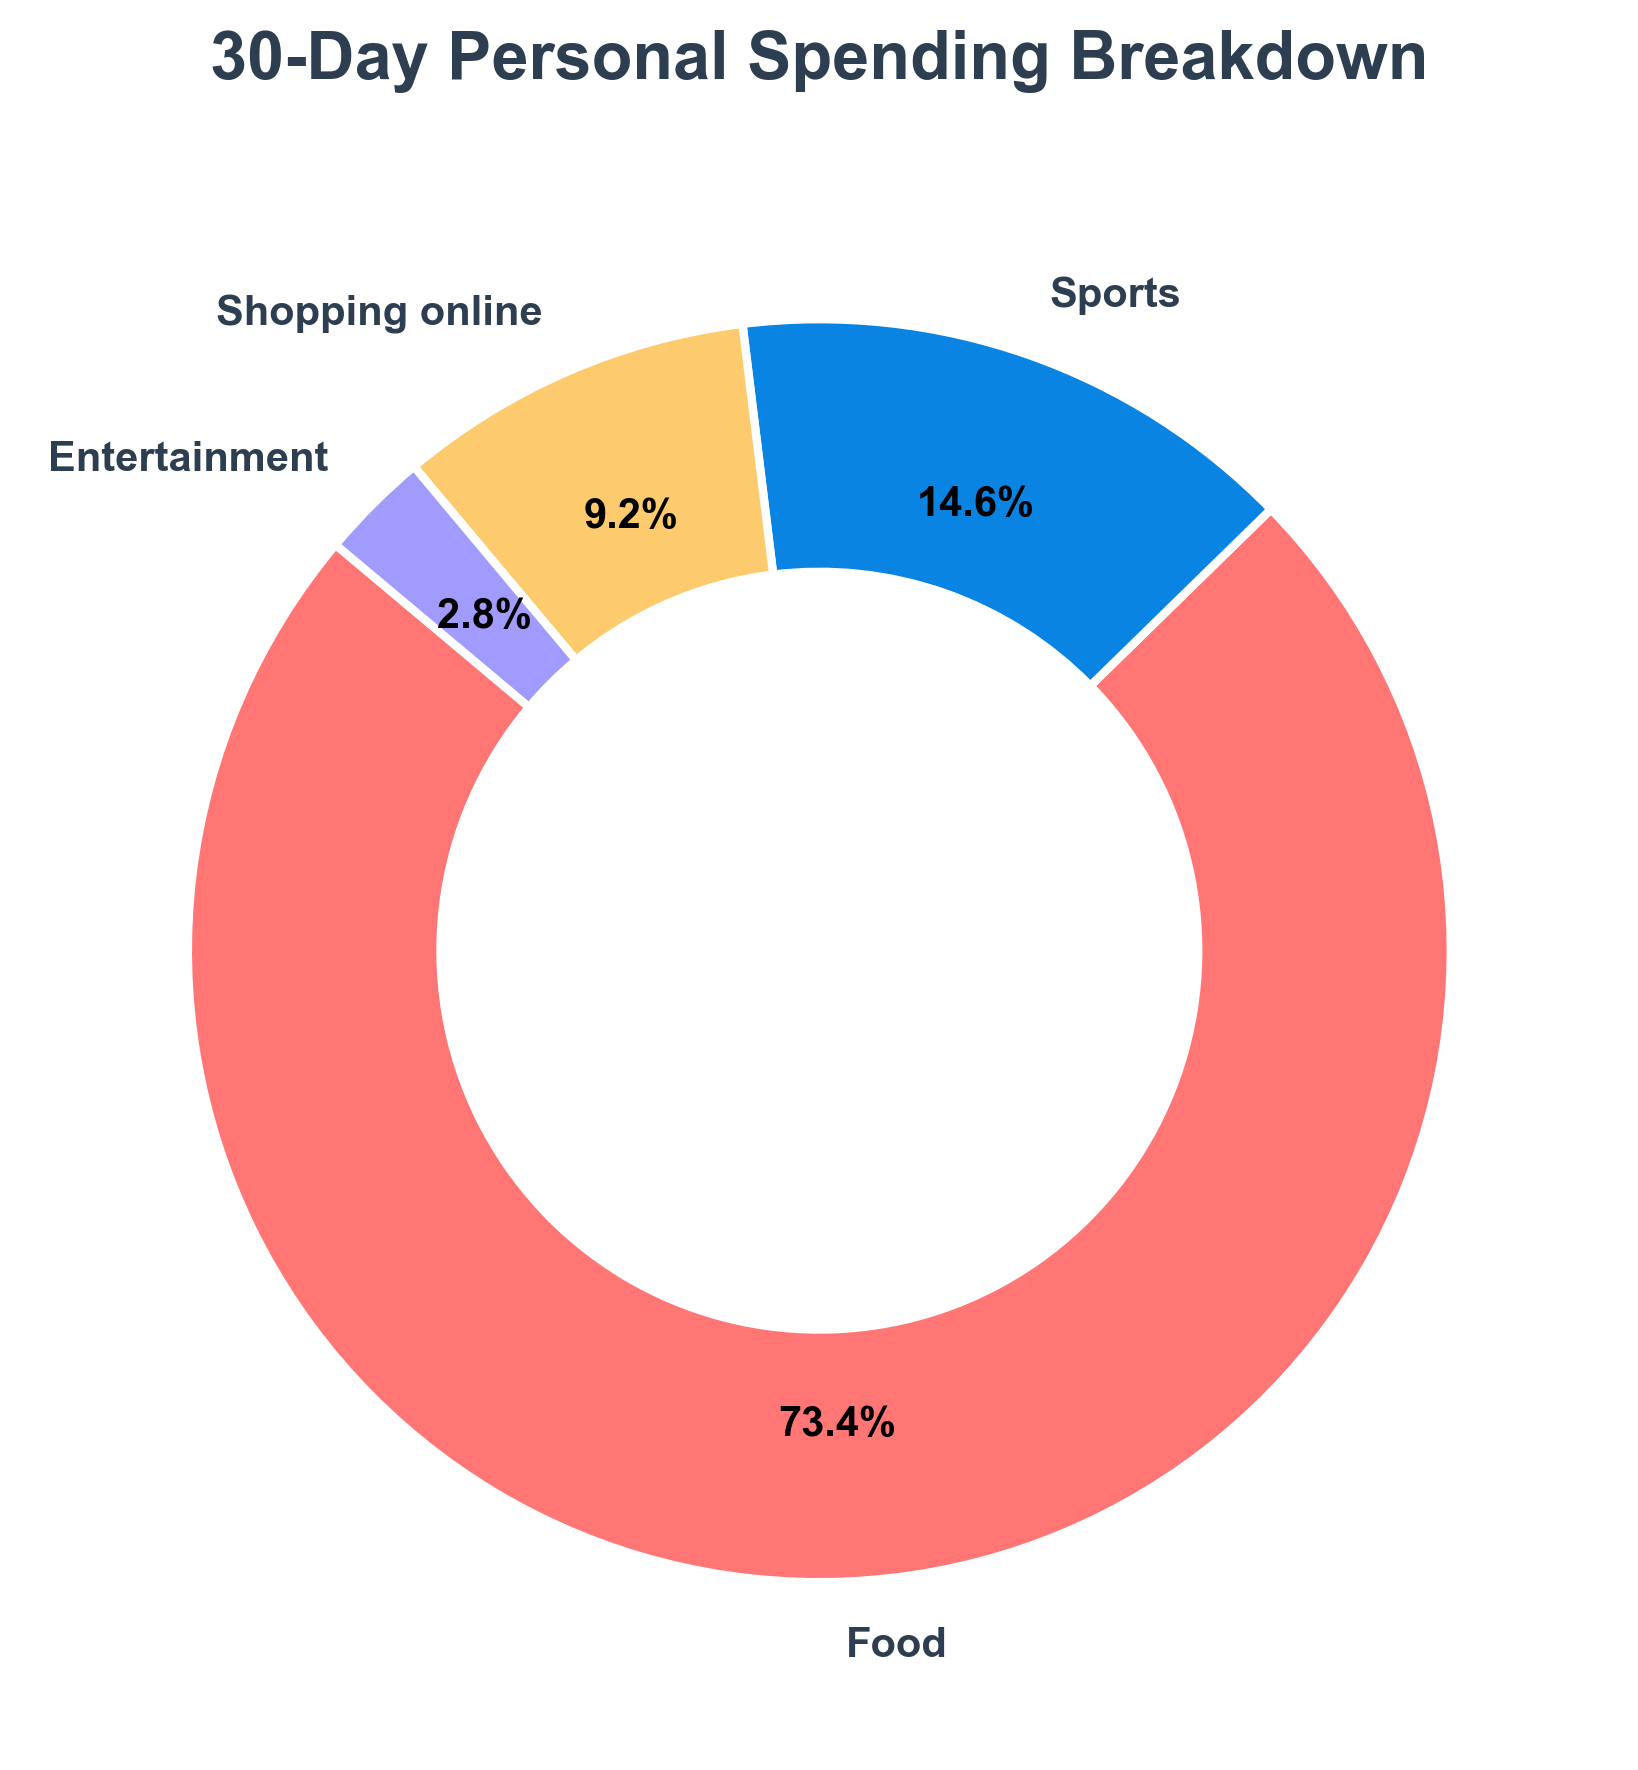
\includegraphics[width=0.40\textwidth]{figures/spending_pie.png}
  \caption{30-day spending by category}
  \label{fig:spending_pie}
  \vspace{-8pt}
\end{wrapfigure}

Food dominates at 73.4\% (3,810,866~VND), split between necessary home groceries from WinCommerce and discretionary dining out and social ``nhậu'' sessions. The discretionary share is the target for reduction. Sports spending at 14.6\% (759,000~VND) covers badminton court bookings and Exbolt~63 restringing at 220,000~VND every two weeks---treated as a committed health cost, not a luxury. Online shopping and entertainment combined account for 12.0\% and are already low, reflecting consistent restraint on non-essential purchases.

\section{Strategic Adjustments}

Two adjustments follow from the data. First, cut dining-out by 30\%---fewer restaurant meals and social drinking sessions, more home cooking. This alone is projected to save over 810,000~VND per month, or 9,700,000~VND per year. Second, share badminton court costs consistently with regular play partners to reduce the per-person sports expense without cutting back on physical activity.

Of the two, the food reduction is the more behaviorally demanding. A large share of the discretionary food spend is tied to social occasions---meals with friends, after-work ``nhậu'' sessions, group outings. These are not purely wasteful; they have real social value. The 30\% target is calibrated to reduce frequency without cutting them out entirely: cooking at home on weekday evenings, treating dining out as a deliberate choice rather than a default, and being more selective about which social occasions are worth the spend. The savings potential is the highest of any category in the budget, and it requires no income increase to realize.

\chapter{Setting SMART Financial Goals}

Saving without a reason is just holding onto cash. I structured my goals using the SMART framework (Specific, Measurable, Achievable, Realistic, Time-bound) across three time windows. Each goal has a defined cost, a funding source, and a hard deadline.

\section{Goal Classification and SMART Matrix}

\subsection{Short-Term Goal (Target: June 2027)}

Two equipment upgrades plus a cash reserve make up the short-term plan. My current ROG Zephyrus G14 laptop is getting slow for professional internship work (data tools, coding, running multiple apps). The target upgrade is a used ThinkPad X1 Carbon Gen~11 (Core i7, 32\,GB RAM, 1\,TB SSD) at 17,000,000~VND, offset by 15,000,000~VND from selling the G14---net cost: 2,000,000~VND. A used Victor Auraspeed 100x Ultra badminton racket (3,000,000~VND) is offset by two trade-ins (1,500,000~VND)---net cost: 1,500,000~VND. On top of these, I want a 20,000,000~VND cash reserve as a basic buffer. Total net capital needed: \textbf{23,500,000~VND}. Saving 2,000,000~VND/month from combined internship and freelance income gets there in 12 months. Target: June 2027.

\begin{takeawaybox}
  \textbf{Short-Term SMART Goals (Target: June 2027)}
  \begin{itemize}[leftmargin=*]
    \item \textbf{Laptop Upgrade:} ThinkPad X1 Carbon Gen 11 (Cost: 17M VND; net outlay: 2M VND after trade-in).
    \item \textbf{Badminton Racket:} Victor Auraspeed 100x (Cost: 3M VND; net outlay: 1.5M VND after trade-ins).
    \item \textbf{Emergency Reserve:} 20M VND liquid cash.
    \item \textbf{Funding Strategy:} Save 2M VND/month from internship and freelance income.
  \end{itemize}
\end{takeawaybox}

\subsection{Medium-Term Goal (Target: December 2030)}

By December 2030, I want two professional qualifications and a solid investment base. The CFA Level~1 exam---the global standard in investment management---costs an estimated 35,000,000~VND including registration and study materials. A Full-Stack Developer certification (ReactJS, NodeJS, cloud deployment) costs 20,000,000~VND and raises the ceiling on my freelance income. The investment target is 100,000,000~VND in liquid assets. Total needed: \textbf{155,000,000~VND}. At a BCG Research Associate salary of 70,000,000~VND/month from 2029, saving 30 to 40\% of after-tax income for 18 months covers all three---alongside continued freelance work.

The two certifications are not interchangeable. CFA Level~1 is the credential that makes me a credible candidate for the analytical and client-facing work BCG expects from a Research Associate. Without it, the application is weaker. The Full-Stack certification serves a different purpose: it raises the value and scope of freelance projects I can take on---moving from simple automation scripts to full application development, which commands significantly higher project fees. Together, they signal to both employers and clients that I can work across the finance-technology boundary, which is increasingly where the most interesting---and best-paid---work sits.

\begin{takeawaybox}
  \textbf{Medium-Term SMART Goals (Target: December 2030)}
  \begin{itemize}[leftmargin=*]
    \item \textbf{CFA Level 1 Exam:} 35M VND total cost (crucial for Research Associate role credibility).
    \item \textbf{Full-Stack Developer Certification:} 20M VND total cost (increases freelance hourly rates).
    \item \textbf{Liquid Investment Base:} 100M VND in broad market index funds.
    \item \textbf{Funding Strategy:} Save 30\%--40\% of BCG fresher salary (70M VND/month gross) over 18 months.
  \end{itemize}
\end{takeawaybox}

\subsection{Long-Term Goal (Target: 2033 \& 2040)}

Two large purchases anchor the long-term plan. First, a Honda Civic e:HEV (costing 900 million VND) in 2033: a down payment of 300 million VND from savings, and a 600 million VND bank loan at 8.0\% over 60 months. The monthly repayment is 12,166,000 VND, representing 10.1\% of my projected monthly income of 120 million VND. Second, a landed house in Thanh Xu\^{a}n, Hanoi (under 50\,m\textsuperscript{2}, under 20 billion VND) in 2040: 10 billion VND personal funds plus a 10 billion VND bank mortgage at 8.5\% over 20 years---monthly repayment: 86.78 million VND (28.9\% of a projected 300 million VND monthly income).

\begin{takeawaybox}
  \textbf{Long-Term SMART Goals (Target: 2033 \& 2040)}
  \begin{itemize}[leftmargin=*]
    \item \textbf{Honda Civic e:HEV (2033):} 900M VND total cost. 300M VND cash + 600M VND loan over 60 months (12.166M VND/month, 10.1\% of gross income).
    \item \textbf{Landed House in Thanh Xuân (2040):} Under 20 billion VND. 10B VND cash + 10B VND mortgage over 20 years (86.78M VND/month, 28.9\% of gross income).
  \end{itemize}
\end{takeawaybox}

\section{Goal Prioritization}

The goals are ordered by dependency: the laptop upgrade supports freelance income today; the certifications unlock the BCG career that funds the car and house; the car responds to family needs at 27; the house is the final long-term wealth store and inflation hedge. Each goal is the step that makes the next one reachable.

\chapter{Personal Financial Statements and Ratio Analysis}

Before deciding where to go, I need to know where I am. This chapter presents my personal balance sheet, income summary, and four financial ratios benchmarked against standard guidelines.

\section{Personal Balance Sheet (as of June 2026)}

\begin{table}[h!]
\caption{Personal Balance Sheet (as of June 2026)}
\label{tab:balance_sheet}
\centering
\begin{tabular}{@{}lrlr@{}}
\toprule
\textbf{Assets} & \textbf{Value (VND)} & \textbf{Liabilities \& Net Worth} & \textbf{Value (VND)} \\
\midrule
\textit{Liquid Assets} & & \textit{Liabilities} & \\
Cash on Hand (ABBank) & 8,000,000 & Current Debt & 0 \\
\textit{Investments} & & Long-term Debt & 0 \\
Stock Portfolio (HOSE) & 28,000,000 & \textbf{Total Liabilities} & \textbf{0} \\
Bitcoin (Crypto)       & 20,000,000 & & \\
\textit{Personal Use Assets} & & & \\
Xiaomi 15 Smartphone   & 11,000,000 & & \\
Datbike Quantum S2     & 43,000,000 & \textbf{Net Worth} & \textbf{126,500,000} \\
ROG Zephyrus G14 Laptop & 16,500,000 & & \\
\midrule
\textbf{Total Assets} & \textbf{126,500,000} & \textbf{Total Liabilities \& NW} & \textbf{126,500,000} \\
\bottomrule
\end{tabular}
\end{table}

\textit{Note.} All personal use assets are valued at current resale market prices.

Total assets are 126,500,000~VND with zero debt. The largest single asset is the Datbike Quantum S2 electric motorcycle, currently valued at 43,000,000 VND. Of the 56,000,000 VND in ``liquid'' assets, only 8,000,000 VND is cash; the remaining 48,000,000 VND is in stocks and Bitcoin, which can drop in value. This is the key weakness addressed in the ratio analysis below.

\section{Income and Expense Summary}

Monthly gross income is 9,500,000~VND from three sources: a fixed internship allowance of 3,000,000 VND from kNowHow Consultant, a monthly family allowance of 4,000,000 VND, and average freelance income of 2,500,000 VND. Monthly out-of-pocket expenses are 5,189,865~VND, leaving a monthly surplus of 4,310,135~VND.

\section{Financial Ratio Analysis}

\begin{enumerate}
  \item \textbf{Savings Ratio:}
    \begin{equation*}
      \text{Savings Ratio} = \frac{4{,}310{,}135}{9{,}500{,}000} \approx 45.4\%
    \end{equation*}
    Benchmark: $>$20\%. Result: 45.4\%---strong, but dependent on not paying rent. If rent were included (4,000,000 to 7,000,000~VND/month), this ratio would be near zero.

  \item \textbf{Liquidity Ratio:}
    \begin{equation*}
      \text{Liquidity} = \frac{56{,}000{,}000}{5{,}189{,}865} \approx 10.8 \text{ months}
      \quad \Rightarrow \quad
      \text{Cash-only} = \frac{8{,}000{,}000}{5{,}189{,}865} \approx 1.5 \text{ months}
    \end{equation*}
    Benchmark: 3--6 months. The headline figure (10.8) looks fine, but cash-only (1.5 months) is below the safe minimum. Building cash reserves to at least 15,000,000~VND is the most urgent action in the near-term plan.

    The distinction between the two numbers matters in practice. If markets fall sharply and I need emergency cash, I cannot rely on selling stocks or Bitcoin at their current stated values---both can lose 30 to 50\% in a downturn, at exactly the moment when cash is most needed. A real emergency fund must be in cash. Until the 15,000,000~VND floor is reached, no additional capital should go into stocks or crypto.

  \item \textbf{Solvency Ratio:}
    \begin{equation*}
      \text{Solvency} = \frac{126{,}500{,}000}{126{,}500{,}000} = 100\%
    \end{equation*}
    Every asset is fully owned---zero debt. Ideal starting point for early wealth-building.

  \item \textbf{Debt Service Ratio:}
    \begin{equation*}
      \text{DSR} = \frac{0}{9{,}500{,}000} = 0\%
    \end{equation*}\nopagebreak[4]
    No monthly debt payments. The full 4,310,135~VND surplus goes to saving and investing. Future debt (vehicle 2033, mortgage 2040) is analyzed in Phases~6 and~7.
\end{enumerate}

\chapter{Personal Income Tax and Career Income Roadmap}

Tax is not optional. Understanding how much of each additional dong goes to the government---and how to legally keep more of it---is one of the most practical skills in personal finance. This phase covers the Vietnamese PIT system and projects my tax bills across five career stages, from student intern to BCG Partner.

\section{Tax Concepts and Definitions}

\textbf{Progressive vs.\ Flat Tax.} A flat tax applies one rate to all income regardless of how much you earn. A progressive tax applies higher rates as income crosses successive brackets. Vietnam's Personal Income Tax (PIT) uses a progressive structure: the more you earn, the higher the rate on each additional increment. The goal is to distribute the tax burden more fairly across income levels.

\textbf{Marginal Tax Rate.} The marginal rate is the rate applied to the next unit of income earned---the rate ``at the margin.'' This is different from the effective tax rate, which is total tax paid divided by total gross income and is always lower. At Stage~2 of my career (BCG Research Associate, 70,000,000~VND/month), my marginal rate will be 30\%, but my effective rate will be only 14.8\%. Why? Because only the income above the last bracket threshold gets taxed at 30\%; lower slices are taxed at 5\%--25\%. People who confuse marginal with effective rates sometimes believe a pay rise will leave them worse off after taxes. It will not.

\textbf{Why This Matters.} As my salary climbs from 70M to 300M~VND/month, proactive planning---registering dependents, making pension contributions, structuring business income through a legal entity---can meaningfully cut my effective rate and increase lifetime after-tax wealth.

\section{The Vietnamese PIT Framework}

Tax residents in Vietnam are subject to a seven-bracket progressive schedule on wages and salaries. The key deduction parameters are: self-deduction 11,000,000 VND/month; dependent deduction 4,400,000 VND/month per registered dependent (children, non-working spouse, or low-income elderly parents); statutory insurance contributions of 10.5\% of gross salary (8\% Social Insurance + 1.5\% Health + 1\% Unemployment), capped at 4,914,000 VND per month; and voluntary pension fund contributions deductible up to 1,000,000 VND/month. The seven PIT brackets are as follows:

\begin{table}[h!]
\caption{Vietnamese Personal Income Tax Brackets (Monthly Taxable Income)}
\label{tab:pit_brackets}
\begin{tabularx}{\linewidth}{@{}rrrX@{}}
\toprule
\textbf{Bracket} & \textbf{Taxable Income (VND/month)} & \textbf{Rate} & \textbf{Tax on this bracket} \\
\midrule
1 & 0 -- 5,000,000            & 5\%  & Up to 250,000 VND \\
2 & 5,000,001 -- 10,000,000   & 10\% & Up to 500,000 VND \\
3 & 10,000,001 -- 18,000,000  & 15\% & Up to 1,200,000 VND \\
4 & 18,000,001 -- 32,000,000  & 20\% & Up to 2,800,000 VND \\
5 & 32,000,001 -- 52,000,000  & 25\% & Up to 5,000,000 VND \\
6 & 52,000,001 -- 80,000,000  & 30\% & Up to 8,400,000 VND \\
7 & Over 80,000,000           & 35\% & No upper cap \\
\midrule
\multicolumn{3}{l}{\textbf{Cumulative tax at top of Bracket 6 (80M taxable)}} & \textbf{18,150,000 VND} \\
\bottomrule
\end{tabularx}
\end{table}



\section{Career Income and PIT Roadmap}

\subsection{Stage 1: Age 20 (2026) --- Intern \& Freelancer}
Gross income is 9,500,000~VND/month. The self-deduction alone (11,000,000~VND) wipes out taxable income entirely. \textbf{PIT owed: 0~VND.} Effective rate: 0.0\%. I am fully exempt at this stage.

\subsection{Stage 2: Age 23 (2029) --- BCG Research Associate (Fresher)}
\begin{itemize}
  \item \textbf{Gross Income:} 70,000,000 VND/month.
  \item \textbf{Deductions:} Self-deduction (11,000,000) + Insurance cap (4,914,000) = 15,914,000 VND.
  \item \textbf{Taxable Income:} 70,000,000 $-$ 15,914,000 = 54,086,000 VND.
  \item \textbf{PIT Calculation (Progressive Brackets):}
    \begin{itemize}
      \item Bracket 1 (0--5M @ 5\%): $5{,}000{,}000 \times 5\% = 250{,}000$ VND
      \item Bracket 2 (5M--10M @ 10\%): $5{,}000{,}000 \times 10\% = 500{,}000$ VND
      \item Bracket 3 (10M--18M @ 15\%): $8{,}000{,}000 \times 15\% = 1{,}200{,}000$ VND
      \item Bracket 4 (18M--32M @ 20\%): $14{,}000{,}000 \times 20\% = 2{,}800{,}000$ VND
      \item Bracket 5 (32M--52M @ 25\%): $20{,}000{,}000 \times 25\% = 5{,}000{,}000$ VND
      \item Bracket 6 (52M--54.086M @ 30\%): $2{,}086{,}000 \times 30\% = 625{,}800$ VND
    \end{itemize}
  \item \textbf{Total PIT Owed:} \textbf{10,375,800 VND/month}. Net income: 59,624,200 VND/month (effective rate: 14.8\%; marginal rate: 30\%).
\end{itemize}

\subsection{Stage 3: Age 28 (2034) --- BCG Consultant (Married, 1 Child)}
\begin{itemize}
  \item \textbf{Gross Income:} 120,000,000 VND/month.
  \item \textbf{Deductions:} Self (11,000,000) + Insurance (4,914,000) + 1 Child (4,400,000) + Pension (1,000,000) = 21,314,000 VND.
  \item \textbf{Taxable Income:} 120,000,000 $-$ 21,314,000 = 98,686,000 VND.
  \item \textbf{PIT Calculation:}
    \begin{itemize}
      \item Brackets 1--5 (up to 52M): 9,750,000 VND
      \item Bracket 6 (52M--80M @ 30\%): $28{,}000{,}000 \times 30\% = 8{,}400{,}000$ VND
      \item Bracket 7 (80M--98.686M @ 35\%): $18{,}686{,}000 \times 35\% = 6{,}540{,}100$ VND
    \end{itemize}
  \item \textbf{Total PIT Owed:} \textbf{24,690,100 VND/month}. Net income: 95,309,900 VND/month (effective rate: 20.6\%; marginal rate: 35\%).
\end{itemize}

\subsection{Stage 4: Age 33 (2039) --- BCG Project Leader (Married, 2 Kids, 2 Dependent Parents)}
\begin{itemize}
  \item \textbf{Gross Income:} 180,000,000 VND/month.
  \item \textbf{Deductions:} Self (11,000,000) + Insurance (4,914,000) + 4 Dependents (17,600,000) + Pension (1,000,000) = 34,514,000 VND.
  \item \textbf{Taxable Income:} 180,000,000 $-$ 34,514,000 = 145,486,000 VND.
  \item \textbf{PIT Calculation:}
    \begin{itemize}
      \item Brackets 1--6 (up to 80M): 18,150,000 VND
      \item Bracket 7 (80M--145.486M @ 35\%): $65{,}486{,}000 \times 35\% = 22{,}920{,}100$ VND
    \end{itemize}
  \item \textbf{Total PIT Owed:} \textbf{41,070,100 VND/month}. Net income: 138,929,900 VND/month (effective rate: 22.8\%; marginal rate: 35\%).
\end{itemize}

\subsection{Stage 5: Age 38 (2044) --- BCG Partner or Tech Founder (Married, 2 Kids, 4 Dependent Parents)}
\begin{itemize}
  \item \textbf{Gross Income:} 300,000,000 VND/month.
  \item \textbf{Deductions:} Self (11,000,000) + Insurance (4,914,000) + 6 Dependents (26,400,000) + Pension (1,000,000) = 43,314,000 VND.
  \item \textbf{Taxable Income:} 300,000,000 $-$ 43,314,000 = 256,686,000 VND.
  \item \textbf{PIT Calculation:}
    \begin{itemize}
      \item Brackets 1--6 (up to 80M): 18,150,000 VND
      \item Bracket 7 (80M--256.686M @ 35\%): $176{,}686{,}000 \times 35\% = 61{,}840{,}100$ VND
    \end{itemize}
  \item \textbf{Total PIT Owed:} \textbf{79,990,100 VND/month}. Net income: 220,009,900 VND/month (effective rate: 26.7\%; marginal rate: 35\%).
\end{itemize}

\section{Tax Optimization Strategies}

Three legal strategies will cut my effective tax rate as income grows. First, register dependents: future children and aging parents reduce taxable income by up to 26,400,000~VND/month (316.8 million VND/year) by age 38. Second, maintain voluntary pension contributions of 1,000,000~VND/month---12 million VND/year in additional deductions. Third, if freelance software work grows enough, establish a registered business entity. This lets me deduct hardware, internet, and office costs before calculating taxable income---a structure that is far more tax-efficient than reporting the same income under the individual progressive schedule.

\chapter{Budgeting and Financial Control}

Tracking spending tells me where money went. Budgeting tells me where it should go. This chapter builds the monthly budget that connects the Phase~1 spending data to the Phase~2 savings goals.

\section{Conceptual Definitions of Expenses}

\textbf{Fixed expenses} are regular, unchanging monthly costs. Mine are just 320,000~VND (internet: 250,000~VND; phone card: 70,000~VND) because my family covers apartment fees, electricity, and water. \textbf{Variable expenses} change based on daily choices: food, sports, shopping, and entertainment. \textbf{Planned expenses} are predictable future costs I can budget for in advance---racket restringing (approx.\ 440,000~VND/month) and shuttlecock purchases (approx.\ 300,000~VND/month). \textbf{Unplanned expenses} are genuine surprises: a clinic visit for a sprained ankle (300,000~VND) and a motorcycle turn signal replacement (300,000~VND) from the tracking period make the case for keeping a monthly emergency buffer.

\begin{table}[h!]
\caption{Classification of Personal Expenses by Type}
\label{tab:expense_classification}
\begin{tabularx}{\linewidth}{@{}p{3cm}p{1.8cm}Xr@{}}
\toprule
\textbf{Category} & \textbf{Type} & \textbf{Controllability} & \textbf{Current Monthly (VND)} \\
\midrule
Internet \& Phone Card  & Fixed    & None --- set by contract    & 320,000   \\
Food (groceries)        & Variable & Medium --- can plan meals   & $\approx$1,200,000 \\
Food (dining out)       & Variable & High --- discretionary      & $\approx$2,600,000 \\
Sports (court \& equipment) & Planned & Medium --- set schedule  & 759,000   \\
Shopping online         & Variable & High --- fully discretionary & 474,999  \\
Entertainment           & Variable & High --- fully discretionary & 145,000  \\
Unplanned (health, moto) & Unplanned & Low --- emergencies       & $\approx$300,000 \\
\midrule
\textbf{Total} & & & \textbf{5,798,999} \\
\bottomrule
\end{tabularx}
\end{table}

The classification reveals an important structural point: almost all of my spending falls into the variable or planned categories, which means almost all of it responds to conscious decisions. Fixed costs---the portion that cannot be changed without switching providers or canceling contracts---represent just 320,000~VND out of roughly 5.8 million in total spending, or 5.5\%. This is unusually low and is almost entirely a result of the family housing arrangement. It also means that virtually every line in my budget is improvable through behavior, not just circumstance. The only category that resists behavioral control is the unplanned one---which is precisely why the 300,000~VND monthly emergency buffer in the target budget exists: not to predict what will go wrong, but to ensure that when something does, it does not come out of next month's savings.



\section{Monthly Target Budget}

\begin{table}[H]
\caption{Monthly Target Budget Structure}
\label{tab:target_budget}
\begin{tabularx}{\linewidth}{@{}lrrL@{}}
\toprule
\textbf{Expense Item} & \textbf{Current (VND)} & \textbf{Target (VND)} & \textbf{Control Strategy} \\
\midrule
Fixed (Internet \& Phone)       & 320,000   & 320,000   & Maintain current plans. \\
Variable --- Food               & 3,810,866 & 3,000,000 & Reduce dining out and social drinking; increase home cooking. \\
Variable --- Sports (Badminton) & 759,000   & 1,000,000 & Health investment. Covers court bookings, shuttlecocks, restringing. \\
Variable --- Shopping online    & 404,999   & 200,000   & Restrict non-essential purchases. \\
Variable --- Entertainment      & 145,000   & 100,000   & Restrict gaming cafe visits and subscriptions. \\
Emergency Buffer                & 0         & 300,000   & Reserve for health or motorcycle maintenance. \\
\midrule
\textbf{Total Expenses} & \textbf{5,439,865} & \textbf{4,920,000} & \\
\bottomrule
\end{tabularx}
\end{table}

Note that sports is budgeted \textit{higher} than current spending (1,000,000 vs.\ 759,000~VND) to cover the full planned cost of court fees, shuttlecocks, and restringing each month. The budget follows a \textbf{35\% Needs / 15\% Wants / 50\% Savings} split. This directs about 4,580,000 VND each month---50.8\% of gross income---to savings, more than twice the standard 20\% benchmark. That margin is enabled almost entirely by not paying rent.

This housing advantage is the defining structural feature of the current budget. It will not last indefinitely: once I move out and pay my own rent---even a modest 5,000,000 to 7,000,000~VND/month room in Hanoi---the savings rate drops to 20 to 25\% at current income, which is still healthy but no longer exceptional. The period between now and when I pay my own rent is therefore the highest-leverage savings window available. Every month of this window that is used well compounds forward; every month wasted does not come back.

\section{Annual Budget Evaluation}

\begin{table}[H]
\caption{Annual Budget Evaluation (12-Month Projection)}
\label{tab:annual_budget}
\begin{tabularx}{\linewidth}{@{}lrrcL@{}}
\toprule
\textbf{Financial Metric} & \textbf{Planned (Year)} & \textbf{Projected (Current)} & \textbf{Met?} & \textbf{Variance Analysis} \\
\midrule
Income   & 114,000,000 & 114,000,000 & Yes & Stable internship, family, and freelance income assumed. \\
Expenses &  59,040,000 &  65,278,380 & No  & Food overspend is the entire source of the gap. \\
Savings  &  54,960,000 &  48,721,620 & Yes & High baseline; full target requires food discipline. \\
\bottomrule
\end{tabularx}
\end{table}

The 6,256,380~VND annual gap between current and target savings is entirely explained by excess food spending. No other category is off-target. Hitting the target budget produces \textbf{54,960,000~VND/year}---enough to fund the equipment upgrades (23,500,000~VND net) and begin the cash emergency fund within the same 12-month window.

\chapter{Personal Credit Strategy}

I currently have no debt and no credit card---a clean position, but also no credit history. Vietnam's CIC (Credit Information Center) system records whether borrowers take out credit products and repay them consistently. Banks and lenders check this record when evaluating any loan application. A borrower with no record at all is treated with caution, because there is no evidence of how they handle debt. Building a score strong enough to support a 10 billion VND mortgage application in 2040 requires a minimum of three to five years of consistent credit card use---which means the first card needs to be opened well before the mortgage is needed.

\section{Building a Credit History}

Three steps, in order. First, get my first credit card in 2029---either a Techcombank Signature or ABBank Visa, with a limit roughly equal to one month's gross salary (50,000,000 to 70,000,000~VND at BCG starting pay). This opens a credit product that generates a repayment record on the CIC system. Second, keep spending below 30\% of the available limit at all times. Banks read low utilization as a sign that I borrow by choice, not out of necessity---a borrower consistently at 80\% of their limit suggests financial stress, while one consistently at 20 to 30\% signals control. Third, set up automatic full-balance payment on the monthly due date. This removes any risk of late-payment marks on the CIC record and requires zero ongoing management after setup.

Two behaviors that significantly damage a CIC score: missing a payment deadline (even by one day) and carrying a revolving balance that accumulates interest. Both are completely avoidable through auto-debit. A clean, unbroken 11-year payment record from 2029 to 2040 is the single strongest signal a Vietnamese bank can receive from a retail mortgage applicant.

\textbf{Practical Example.} The Vietcombank VCB Visa Classic is a strong first card: initial limit of 10,000,000 to 50,000,000~VND for verified-salary applicants, 45-day interest-free period, auto-debit payment available through VCB digital banking, and accepted at virtually every merchant and online platform in Vietnam. Spending under 15,000,000~VND/month on a 50,000,000~VND limit and paying automatically builds a clean CIC record within 12 months of activation. Starting in 2029 gives 11 years of documented credit history before the 2040 mortgage application.

\section{Long-Term Debt Strategy}

For the Thanh Xu\^{a}n house in 2040: total price 20,000,000,000~VND, split 50-50 between personal funds and bank debt. The 10,000,000,000~VND bank loan runs over 240 months at an estimated 8.5\% per annum, producing a monthly payment of approximately \textbf{86,780,000~VND}. At a projected income of 300,000,000~VND/month as BCG Partner, this is a Debt Service Ratio of 28.9\%---below the 35\% safe lending ceiling used by Vietnamese banks.

The 50\% Loan-to-Value ratio provides a meaningful equity buffer. If property prices fall during the 20-year repayment period, the outstanding loan balance remains below the property value as long as prices do not drop more than 50\% from the 2040 purchase level---an extremely unlikely scenario for a well-located house in an urban district of Hanoi. The combination of a strong CIC record, a verified high income at BCG salary levels, and a 50\% down payment means the mortgage application in 2040 should be approved at competitive rates. The credit-building work that starts in 2029 is what makes the 2040 application straightforward rather than difficult.

\chapter{Vehicle Purchase Strategy}

Buying a family car is planned for 2033. Unlike a house, a vehicle depreciates from the moment it leaves the showroom---and continues to lose value every year regardless of how well it is maintained. Getting the decision right means not just picking the right vehicle, but choosing the right method of acquiring it and understanding what it truly costs to own per month. This phase compares all three acquisition options, selects the best fit for my circumstances, and calculates total monthly ownership cost.

\section{Comparison of Acquisition Options}

\begin{table}[h!]
\caption{Comparison of Vehicle Acquisition Options}
\label{tab:vehicle_options}
\begin{tabularx}{\linewidth}{@{}lLLL@{}}
\toprule
\textbf{Factor} & \textbf{Lease} & \textbf{New Purchase} & \textbf{Used Purchase} \\
\midrule
Upfront Cost   & Low or none & High down payment & Lower down payment \\
Monthly Cost   & Lower fixed payment & Higher loan repayment & Lower loan repayment \\
Ownership      & No ownership at end & Full ownership & Full ownership \\
Depreciation Risk & Borne by lessor & High: 30--40\% Year 1 & Low: already depreciated \\
Maintenance    & Often included & Owner's full responsibility & Owner's full responsibility \\
Flexibility    & Mileage caps; no modifications & Keep, modify, or sell freely & Keep, modify, or sell freely \\
Best For       & Short-term, business use & Long-term family ownership & Budget-conscious buyers \\
\bottomrule
\end{tabularx}
\end{table}

\textbf{Why not lease?} Leasing ends without ownership---every payment builds equity in the vehicle, then hands it back at contract end. For business users who need a new vehicle every two to three years and can deduct lease costs, this makes sense. For a young family planning to keep a car for seven to ten years in Hanoi, it does not. The cumulative lease payments over a decade would likely exceed the outright purchase cost, with nothing to show for it at the end.

\textbf{Why not used?} A 3-year-old Honda Civic of equivalent specification typically trades at 650,000,000 to 700,000,000~VND in Vietnam's secondary market---a 22 to 28\% discount to the 900,000,000~VND new price. That is a real saving. However, two constraints make it the wrong choice specifically in this plan: first, used hybrid models are rare in Vietnam---the Honda Civic e:HEV is not yet widely traded second-hand, which limits selection and raises overpayment risk; second, any used vehicle bought in 2033 is at least three years old with an expired factory warranty, inheriting mechanical risk at exactly the life stage when reliability matters most.

\textbf{Selected: New Purchase.} Full manufacturer warranty, complete service history from day one, and access to the latest hybrid or EV efficiency technology. At BCG Consultant income levels in 2033, the premium over a used purchase is manageable and the peace-of-mind value is high.

\section{Vehicle Specifications and Financing}

Target: Honda Civic e:HEV (Hybrid 5-seater sedan) or VinFast VF7 (Electric SUV) at approximately 900,000,000~VND. Financing structure: 300,000,000~VND down payment (33\%), 600,000,000~VND bank loan at 8.0\% per annum over 60 months. Monthly loan repayment: approximately \textbf{12,166,000~VND}. At a projected income of 120,000,000 VND per month as BCG Consultant in 2033, this is 10.1\% of gross income---well within the 15\% vehicle debt ceiling. The 33\% down payment is deliberately above the typical 20 to 25\% bank minimum: a larger equity stake from day one reduces the risk of being underwater on the loan if resale value drops faster than expected in the first two years.

\section{Total Cost of Ownership}

\begin{table}[h!]
\caption{Monthly Vehicle Running Costs}
\label{tab:vehicle_tco}
\begin{tabularx}{\linewidth}{@{}lrL@{}}
\toprule
\textbf{Cost Item} & \textbf{Monthly (VND)} & \textbf{Notes} \\
\midrule
Fuel / Electricity      & 1,500,000 & Hybrid/EV saves 500,000--1,000,000 vs.\ petrol equivalent \\
Maintenance / Battery   & 1,200,000 & Scheduled service or VinFast battery lease fee \\
Parking \& Tolls        & 1,300,000 & Monthly parking in Hanoi + urban road tolls \\
Insurance \& Registration & 1,000,000 & Civil liability + optional comprehensive (amortized) \\
\midrule
\textbf{Total Running Costs} & \textbf{5,000,000} & \\
\textbf{Total Monthly (Loan + Running)} & \textbf{17,166,000} & 14.3\% of projected 120M income \\
\bottomrule
\end{tabularx}
\end{table}

The 14.3\% total vehicle cost as a share of income sits just below the standard 15\% guideline for vehicle debt. The hybrid or electric engine choice reduces the fuel line significantly compared to a conventional petrol sedan of similar size---a petrol alternative in Hanoi traffic would typically cost 2,000,000 to 2,500,000~VND/month in fuel, making the hybrid or EV option approximately 500,000 to 1,000,000~VND cheaper to run per month over a five-year ownership period.

\chapter{Investment Strategy and Stock Analysis}

Money in a savings account barely keeps up with inflation (3 to 4\% per year in Vietnam). Building real wealth requires putting money into productive assets that earn more than inflation. This phase analyzes Binh Dien Fertilizer Joint Stock Company (BFC) on HOSE as the target for a 200,000,000~VND stock investment.

\section{Company Profile}

BFC was set up in 1973, converted to a joint-stock company, and listed on HOSE in 2015. Today it is the leading NPK fertilizer maker in Vietnam by market share. Its strong market position comes from 50 years of distribution network development and the ``\DH\`{a}u Tr\^{a}u'' (Buffalo Head) brand---a name Vietnamese farmers across the Mekong Delta and Central Highlands have trusted for generations. Brand loyalty in fertilizer is especially strong because farmers do not switch products in a growing season: the perceived risk to their crop is too high. BFC also sells bio-organic fertilizers, foliar fertilizers, and agricultural advice services.

From a portfolio fit perspective, BFC complements my other assets. My Bitcoin holding (valued at 20,000,000 VND) is high-risk and volatile. The stock portfolio on HOSE (28,000,000 VND) and freelance income both go up and down. BFC adds regular, predictable cash dividends---paid regardless of what broader markets are doing---which stabilizes the overall portfolio.

\section{Financial Snapshot (FY2024)}

BFC's 2024 results beat expectations across all key measures. Total net revenues: 9,489 billion~VND, up 9.0\% year-on-year and 33\% above the company's own annual target. Net income: 425.6 billion~VND, with Profit Before Tax up 170.6\% vs.\ 2023. Cash dividends for 2024: 30\% (3,000~VND/share), giving a yield of approximately 5.2\% at the current price of 57,300~VND/share (June~4, 2026). Trailing P/E: approximately 7.7$\times$ (estimated EPS: 7,445~VND)---roughly half the VN-Index average of approximately 14$\times$. Shares outstanding: 57,167,993. BFC outperformed the VN-Index over 2024 to 2026.

The combination of a 5.2\% dividend yield and a 7.7$\times$ P/E deserves specific attention. A 5.2\% yield means the stock pays roughly the same annual cash return as a 12-month bank deposit at most major Vietnamese commercial banks---except that it also carries the possibility of capital appreciation if the market re-rates BFC closer to its fair value. The 170.6\% growth in Profit Before Tax in 2024 is not typical for an established agricultural company; it reflects real operational improvement, not an accounting adjustment. At a P/E of 14$\times$ (the market average), BFC would trade at approximately 104,000~VND/share---an 81\% premium to its current price. Even a partial re-rating represents a meaningful capital gain on top of the dividend income.

\section{Investment Thesis (VND 200,000,000 Allocation)}

At 57,300~VND/share, 200,000,000~VND buys \textbf{3,490 shares}. Four reasons support this investment:

\textbf{1. Cheap valuation.} A P/E of 7.7$\times$ on record earnings suggests the market has not fully repriced the stock after the 2024 earnings improvement. Even a re-rating to 10$\times$ earnings---still below market average---represents a 30\% price gain.

\textbf{2. Steady dividend income.} At 3,000 VND per share per year, 3,490 shares produce annual cash dividends of \textbf{10,470,000 VND}. This income is paid regardless of daily price movements and compounds into a larger holding when reinvested.

\textbf{3. Durable brand position.} The ``\DH\`{a}u Tr\^{a}u'' brand cannot be taken away by a new product or a price cut. It has been built over 50 years in the most productive farming regions of the country.

\textbf{4. Right portfolio role.} BFC is the stable, income-generating anchor that counterbalances Bitcoin's price swings. Low link to crypto markets; tied instead to Vietnam's farming economy.

\section{Key Investment Risks}

\begin{table}[h!]
\caption{BFC Investment Risk Summary}
\label{tab:bfc_risks}
\begin{tabularx}{\linewidth}{@{}lLL@{}}
\toprule
\textbf{Risk} & \textbf{Description} & \textbf{Monitoring Approach} \\
\midrule
Raw Material Costs & BFC imports Urea, DAP, and Potassium on global commodity markets. Input cost spikes not passed on to customers compress margins. & Track quarterly gross margin trend in earnings reports. Sell if margin falls below 8\% for two consecutive quarters. \\[6pt]
Weather / Climate & Revenue is directly tied to farming activity. Droughts, flooding, or saltwater intrusion in key provinces reduce fertilizer demand. & Monitor annual MARD (Ministry of Agriculture) crop output data. Cannot be hedged; must be accepted as a structural feature. \\[6pt]
Competitive Pressure & PVCFC, DPM, and Lâm Thao compete domestically; Chinese imports compete on price. Margin pressure could slow dividend growth. & Track BFC market share in annual reports. ``\DH\`{a}u Tr\^{a}u'' brand loyalty provides a buffer, but not permanent protection. \\
\bottomrule
\end{tabularx}
\end{table}

Of the three, raw material cost volatility is the most immediately trackable and the one most likely to produce a short-term price drop. Weather and competitive risks are slower-moving and more structural---they affect long-term dividend growth rather than creating sharp short-term earnings declines. None of the three risks invalidates the investment thesis at a 7.7$\times$ P/E entry point, where the stock is already priced as though the business has limited growth prospects. They are risks to monitor, not reasons to avoid the position.


\chapter{Personal Risk Management and Insurance Strategy}

A financial plan assumes things go as expected. When they do not---a medical bill, a broken motorcycle, a missed freelance payment---the plan needs a way to absorb the hit without wiping out months of savings. Risk management here works at two levels: a cash buffer for ordinary disruptions, and insurance for larger, less predictable events.

\section{Emergency Fund Plan}

My current risk coverage across four areas: health is covered by the mandatory student Bảo hiểm Y tế (BHYT) for public hospitals plus a Bảo Việt An Gia Silver private plan (private hospitals, direct billing); income disruption risk is managed through three concurrent sources (no single source is more than 42\% of total income); the Datbike Quantum S2 has vehicle accident insurance; the family apartment has no rental exposure on my side.

The remaining gap is cash. Emergency fund target: \textbf{30,000,000~VND} (approximately 6 months of expenses at the 4,920,000~VND/month target budget), held entirely in cash or short-term bank deposits---not stocks or Bitcoin. Current cash-only cover is only 1.5 months (see Phase~3). Building this fund runs in parallel with the equipment upgrade goal.

\section{Insurance Coverage by Life Stage}

\begin{table}[h!]
\caption{Insurance Planning by Life Stage}
\label{tab:insurance_stages}
\begin{tabularx}{\linewidth}{@{}lLL@{}}
\toprule
\textbf{Life Stage} & \textbf{Insurance Coverage Needed} & \textbf{Rationale} \\
\midrule
Student (Ages 18--22)   & Mandatory student Bảo hiểm Y tế (BHYT) + Bảo Việt An Gia & Low-cost access to private clinics alongside public BHYT cover. \\[6pt]
First Job (Ages 23--27) & Employer-provided group health insurance (BCG benefit) & Full medical, dental, and outpatient cover funded by employer. \\[6pt]
Mid-Career (Ages 28+)   & Term Life + Critical Illness Insurance & Protects family dependents if the main earner dies or can no longer work. \\
\bottomrule
\end{tabularx}
\end{table}

At each stage, the type of risk that matters most changes. As a student with no dependents, the main risk is a large personal medical bill. At BCG, employer insurance covers this at no extra cost. From age 28, with a spouse, children, and aging parents depending on my income, the risk shifts to the family losing its main income source---which term life and critical illness insurance are designed to address.

\section{Evaluated Insurance Policy}

Selected: \textbf{Bảo Việt An Gia Silver Package}. Annual premium: 2,500,000 VND per year (approximately 208,000 VND per month). Coverage: inpatient and surgery up to 90,000,000 VND per year (surgery sub-limit: 45,000,000 VND); room and board up to 4,500,000 VND per day; direct billing at Hong Ngoc, Thu Cuc, and Vinmec hospitals in Hanoi. At 208,000 VND per month, this plan removes the need to pay upfront at private hospitals and covers most realistic medical events in Vietnam---making it one of the best-value decisions in this entire plan.

To see why this is worth 208,000 VND per month, consider what Bảo hiểm Y tế (BHYT) only coverage means in practice. BHYT sends patients to public hospitals, where outpatient queues commonly run two to four hours, shared wards are standard for inpatient stays, and access to specialist care requires an internal referral process that can add days to a diagnosis. For a student whose income depends on consistently showing up to an internship and delivering freelance projects on time, a two-day delay in getting a diagnosis is not just uncomfortable---it has a direct cost in lost work. The Bảo Việt An Gia plan allows same-day appointments at private hospitals with direct specialist access and no upfront payment. For 208,000 VND per month, it converts a potentially multi-day health disruption into a two-hour clinic visit.

Two practical renewal considerations: first, this plan should be reviewed annually. If the hospital network changes or new private health plans with better coverage-to-premium ratios become available, switching at renewal costs nothing. Second, when joining BCG after graduation in 2029, the employer group health insurance will replace this plan at zero personal cost. At that point, the personal Bảo Việt An Gia policy should be cancelled---there is no benefit in paying twice for overlapping coverage.


\chapter{Retirement Planning and Compounding Strategy}

Most people understand that saving for retirement matters. Very few understand how much it matters \textit{when} they start. At a 9\% annual return: 1,500,000~VND/month saved from age 20 grows to approximately \textbf{6.6 billion VND} by age 60. The same amount saved from age 35 grows to only about \textbf{1.5 billion VND}. The 15-year head start produces more than four times the result---from the same monthly amount. Starting at 20, even with small amounts, matters far more than starting large at 35.

\section{Retirement Parameters (Questions 10.1--10.4)}

\begin{description}
  \item[\textbf{10.1 --- Retirement Age Target:}] \textbf{60 years old.} More than 30 years of formal employment covers the full BHXH contribution period for maximum state pension. At 60, I am still young enough to travel, play badminton, and spend real time with family.

  \item[\textbf{10.2 --- Expected Years After Retirement:}] \textbf{25 years} (ages 60 to 85). Vietnam's male life expectancy is currently around 73 years, but planning to 85 is the right safe assumption with access to private healthcare over a long career.

  \item[\textbf{10.3 --- Desired Retirement Lifestyle:}] \textbf{Comfortable.} Two to three trips per year (domestic and international), regular sport, access to private healthcare without cost anxiety, and financial capacity to support adult children when needed.

  \item[\textbf{10.4 --- Monthly Income Needed:}] \textbf{15,000,000~VND/month} in today's money, covering housing upkeep, healthcare, travel, food, recreation, and family spending. Funded primarily by rental income, stock dividends, and the BHXH state pension.
\end{description}

\textbf{Compounding.} The math: $1.09^{40} \approx 31.4$ versus $1.09^{15} \approx 3.6$. Investing at 20 earns 8.7$\times$ more per dong than investing at 45, from the same annual return. Stage~1 (ages 20--22) starts the compounding clock 15 years earlier than it would otherwise; those first 15 years produce a much larger share of the final total than the same 15 years would at any later point.

\section{Multi-Stage Saving Strategy}

\textbf{Stage 1 (Ages 20--22):} Allocate 1,500,000~VND/month to BFC stock and Bitcoin while building the 30,000,000~VND emergency fund from the 4,310,135~VND monthly surplus. Both goals run in parallel.

\textbf{Stage 2 (Ages 23--45):} The main wealth-building phase. BCG salary grows from 70,000,000 to 300,000,000~VND/month. Saving 20 to 30\% of after-tax income generates capital flows far beyond anything possible during the student years. Key milestones: car purchase (2033, financed), Thanh Xuân house (2040, mortgaged), reinvestment of all BFC dividends, and rental income accumulation. Goal: a portfolio large enough to produce a passive monthly income of 15,000,000 VND without salary dependency.

To put the Stage~2 numbers in context: at a BCG Consultant monthly income of 120,000,000 VND (age 28), saving 25\% of after-tax income---approximately 22,000,000 VND per month after tax and deductions---compounds to over 2 billion VND over 10 years at a 9\% annual return, without accounting for salary growth. As the salary grows toward 300,000,000~VND/month, the investable surplus grows proportionally. The 300,000,000~VND down payment for the Thanh Xuân house in 2040 is not a stretch target at that income level; it is a conservative one. The critical discipline in Stage~2 is not earning more---that is already planned---but not inflating lifestyle expenses at the same rate as income grows.

\textbf{Stage 3 (Ages 46--60):} Pay off the house mortgage early if possible. Gradually shift the portfolio from growth assets toward stable income-paying ones (dividend stocks, government bonds, short-term deposits) to reduce risk as retirement approaches.

\section{Retirement Income Streams}

At age 60, the 15,000,000~VND/month target comes from four sources: \textbf{rental income} from the Thanh Xuân property (growing with inflation, projected to cover the full target alone by 2060); \textbf{BFC dividends} from the accumulated portfolio reinvested throughout the saving years; \textbf{BHXH state pension} from 30+ years of social insurance contributions at BCG salary levels; and \textbf{Bitcoin sales} used as a flexible reserve---sold in small amounts to supplement other sources as needed rather than as a primary income stream. The mix is deliberate: no single bad event---a property downturn, a dividend cut, a pension reform, or a crypto collapse---can shut down all four at once.


%% Conclusion (unnumbered)
\chapter*{Conclusion and Personal Commitment}
\addcontentsline{toc}{chapter}{Conclusion and Personal Commitment}

This plan was built from real data---67 actual bank transactions, a balance sheet at current resale values, five stages of PIT calculation, and a retirement compound-growth model using specific numbers. Its value is not that it predicts the future precisely. Its value is that it connects today's small decisions to outcomes 20, 30, and 40 years from now.

The spending analysis in Phase~1 showed a savings rate of 45.4\%---strong, but backed by a cash-only liquidity of just 1.5 months. The most urgent near-term action is not saving more, but moving part of existing savings into a dedicated cash reserve of at least 15,000,000 to 30,000,000~VND. The three tiers of goals in Phase~2 are ordered by dependency: the laptop upgrade supports freelance income now; the CFA and coding certifications unlock the BCG salary; the BCG salary funds the car and the house. Cut the link at any point and everything after it shifts.

The tax analysis in Phase~4 shows that effective rates rise from 0\% today to 14.8\%, 20.6\%, 22.8\%, and 26.7\% across career stages---but never hit the 35\% top bracket because dependent deductions, insurance contributions, and pension contributions keep taxable income below the ceiling. Registering two children and two dependent parents alone reduces taxable income by up to 316,800,000~VND/year. The budget in Phase~5 shows that the entire 6.2-million-VND annual savings gap is caused by one behavior---dining out too often---and needs no income increase to fix.

The BFC investment (Phase~8) handles the risk of money not growing fast enough. The Bảo Việt An Gia policy at 208,000~VND/month (Phase~9) handles the risk of a single health event wiping out what has been saved. Both risks are real; neither is optional to manage. The retirement math in Phase~10 makes the case for starting now: the same 1,500,000~VND/month invested at 20 versus 35 produces 6.6 billion VND versus 1.5 billion VND by age 60---four times the result, from the same monthly contribution, purely because of the time difference.

This plan will change as life does. But the framework---tracking spending, setting goals, understanding tax, using credit carefully, insuring against major risks, investing early, planning for retirement---stays valid regardless of how the numbers shift. That framework is what this report delivers.


%% References (APA: after body, before appendices)
%% APA 7th Edition References
%% Format: hanging indent 1.27 cm (0.5 inch), alphabetical by first author surname
\chapter*{References}
\addcontentsline{toc}{chapter}{References}

\sloppy   %% allow flexible spacing to prevent URL overflow
\begin{hangparas}{1.27cm}{1}

Bao Viet Insurance. (2025). \textit{Bao Viet An Gia health insurance: Benefits and coverage guide}. \url{https://www.baoviet.com.vn/insurance/bao-viet-an-gia}

Binh Dien Fertilizer Joint Stock Company. (2025). \textit{Audited consolidated financial statements for the fiscal year ended December 31, 2024}. \url{https://binhdien.com/quan-he-co-dong/bao-cao-tai-chinh}

Boston Consulting Group. (2026). \textit{Careers in consulting: Research Associate and Consultant roles in Vietnam}. \url{https://www.bcg.com/careers}

National Assembly of Vietnam. (2007). \textit{Law on Personal Income Tax} (Law No.~04/2007/QH12). Ministry of Finance. \url{http://vanban.chinhphu.vn}

National Assembly of Vietnam. (2012). \textit{Law amending and supplementing a number of articles of the Law on Personal Income Tax} (Law No.~26/2012/QH13). Ministry of Finance. \url{http://vanban.chinhphu.vn}

State Bank of Vietnam. (2026). \textit{Regulations on credit scores and banking interest rates in Vietnam}. \url{https://sbv.gov.vn}

Vietnam Ministry of Finance. (2013). \textit{Circular No.~111/2013/TT-BTC guiding the implementation of the Law on Personal Income Tax and Decree No.~65/2013/ND-CP}. \url{http://mof.gov.vn}

Vietnam Social Security. (2025). \textit{Statutory social insurance, health insurance, and unemployment insurance contribution rates and caps for 2025/2026}. \url{https://baohiemxahoi.gov.vn}

Vietstock Finance. (2026). \textit{BFC -- Binh Dien Fertilizer Joint Stock Company: Stock profile and financial ratios}. \url{https://finance.vietstock.vn/BFC-ctcp-phan-bon-binh-dien.htm}

\end{hangparas}
\fussy   %% restore normal spacing after references


%% Appendix
\appendix
\chapter{Raw Transaction Logs}

\section{Daily Expenditure Logs (May 7 -- June 4, 2026)}

{\small\centering
\begin{longtable}{lp{6.2cm}lr}
\caption{Daily Expenditure Logs (May~7 -- June~4, 2026)} \label{tab:daily_logs} \\
\toprule
\textbf{Date} & \textbf{Payee / Description} & \textbf{Category} & \textbf{Amount (VND)} \\
\midrule
\endfirsthead
\toprule
\textbf{Date} & \textbf{Payee / Description} & \textbf{Category} & \textbf{Amount (VND)} \\
\midrule
\endhead
\midrule
\multicolumn{4}{r}{\textit{Continued on next page}} \\
\endfoot
\bottomrule
\endlastfoot
07/05/2026 & WINCOMMERCE JSC                       & Food            &  94,900 \\
07/05/2026 & Phone credit top-up (0834781535)      & Shopping        &  50,000 \\
07/05/2026 & Phone credit top-up (0834781535)      & Shopping        &  20,000 \\
07/05/2026 & NGHIEM DUC TRUNG -- court booking     & Sports          & 120,000 \\
07/05/2026 & CPN THUAN PHONG -- delivery fee       & Shopping        & 150,000 \\
08/05/2026 & MAI VAN TUAN                          & Food            & 500,000 \\
08/05/2026 & LU VAN NHO                            & Food            & 175,000 \\
09/05/2026 & NGUYEN DOAN NGUYEN AN                 & Shopping        & 199,999 \\
09/05/2026 & GS25                                  & Food            & 167,000 \\
09/05/2026 & SPARTACUS GAMING CENTER               & Entertainment   &  55,000 \\
10/05/2026 & VU THI PHIEN                          & Food            &  45,000 \\
12/05/2026 & Phone credit top-up (0855121006)      & Shopping        &  10,000 \\
12/05/2026 & CHA BA LUA                            & Food            &  25,000 \\
12/05/2026 & DO THI NGA                            & Food            & 195,000 \\
13/05/2026 & DANG THAI HOC                         & Food            &  40,000 \\
13/05/2026 & LU VAN NHO                            & Food            & 290,000 \\
13/05/2026 & WINCOMMERCE JSC                       & Food            &  21,300 \\
14/05/2026 & CHA BA LUA                            & Food            &  25,000 \\
15/05/2026 & TRAN THI THUY                         & Food            &  45,000 \\
15/05/2026 & SIEU THI THANH DO 12 KHUAT DUY TIEN   & Food            & 112,136 \\
15/05/2026 & BUI VAN QUANG                         & Food            &  35,000 \\
16/05/2026 & MOMO ANH                              & Entertainment   &  10,000 \\
16/05/2026 & MOMO                                  & Entertainment   &  80,000 \\
17/05/2026 & WINCOMMERCE JSC                       & Food            &  45,920 \\
17/05/2026 & WINCOMMERCE JSC                       & Food            & 132,800 \\
17/05/2026 & WINCOMMERCE JSC                       & Food            &  55,000 \\
18/05/2026 & NGUYEN HOANG ANH                      & Food            &  48,000 \\
19/05/2026 & DO THI NGA                            & Food            & 165,000 \\
19/05/2026 & DANG THAI HOC                         & Food            &  40,000 \\
20/05/2026 & DINH THI LY                           & Food            &  45,000 \\
20/05/2026 & GS25                                  & Food            &  68,000 \\
21/05/2026 & CHA BA LUA                            & Food            &  25,000 \\
21/05/2026 & NGUYEN VAN DUC                        & Food            &  20,000 \\
22/05/2026 & PHAN HOANG VIET                       & Food            &  45,000 \\
22/05/2026 & BAOKIM TH103                          & Shopping        &   5,000 \\
22/05/2026 & TRUONG DU KY -- court booking         & Sports          & 140,000 \\
22/05/2026 & NGUYEN HUONG GIANG                    & Food            &   5,000 \\
22/05/2026 & HO KD HOANG LE NGOC BAO               & Shopping        &  40,000 \\
23/05/2026 & BUN RIEU CUA MADAME VAN               & Food            &  40,000 \\
23/05/2026 & TRUONG VAN HAI                        & Food            & 153,000 \\
23/05/2026 & WINCOMMERCE JSC                       & Food            &  97,420 \\
24/05/2026 & SAN CAU LONG 686                      & Sports          & 340,000 \\
24/05/2026 & NGUYEN THI DIEM                       & Food            &  50,000 \\
25/05/2026 & BUI VAN QUANG                         & Food            &  40,000 \\
25/05/2026 & DO VAN DOAN                           & Food            &  17,000 \\
26/05/2026 & NGUYEN THAI SON                       & Food            &  55,000 \\
26/05/2026 & LE PHUONG THAO                        & Food            &  40,000 \\
27/05/2026 & GS25                                  & Food            &  24,000 \\
27/05/2026 & NGUYEN THI THU THUY                   & Food            &  22,000 \\
27/05/2026 & CONG TY CP DICH VU VAN HOA THE THAO   & Sports          &  39,000 \\
27/05/2026 & HO KINH DOANH PHO CO                  & Food            &  45,000 \\
28/05/2026 & DINH THI LY                           & Food            &  45,000 \\
29/05/2026 & SIEU THI THANH DO 12 KHUAT DUY TIEN   & Food            & 156,490 \\
29/05/2026 & WINCOMMERCE JSC                       & Food            &  98,900 \\
29/05/2026 & LU VAN NHO                            & Food            & 125,000 \\
30/05/2026 & BUI VAN QUANG                         & Food            &  40,000 \\
30/05/2026 & NGHIEM DUC TRUNG -- court booking     & Sports          &  80,000 \\
31/05/2026 & GS25                                  & Food            &  31,000 \\
31/05/2026 & NGHIEM DUC TRUNG -- court booking     & Sports          &  40,000 \\
01/06/2026 & PHAM VAN DIEP                         & Food            &  48,000 \\
02/06/2026 & DANG THAI HOC                         & Food            &  45,000 \\
03/06/2026 & PHAN QUANG HIEU                       & Food            &  33,000 \\
04/06/2026 & NGUYEN TRINH GIA HAN                  & Food            &  70,000 \\
04/06/2026 & NGUYEN THI ANH TUYET                  & Food            &  25,000 \\
04/06/2026 & BUI VAN QUANG                         & Food            &  45,000 \\
\end{longtable}
}

\textit{Note.} All 67 transactions exported from ABBank mobile banking (May~7 -- June~4, 2026). Descriptions are lightly abbreviated for readability.

%% ── A.2 and A.3 side by side ──────────────────────────────
\section{Category Summary and Income Trajectory}

\noindent
\begin{minipage}[t]{0.44\linewidth}
  \captionsetup{type=table}
  \caption{Spending Totals by Category}
  \label{tab:category_totals}
  \vspace{4pt}
  \centering\small
  \begin{tabular}{@{}lrr@{}}
  \toprule
  \textbf{Category} & \textbf{Total (VND)} & \textbf{Share} \\
  \midrule
  Food            & 3,810,866 & 73.4\% \\
  Sports          &   759,000 & 14.6\% \\
  Shopping online &   474,999 &  9.2\% \\
  Entertainment   &   145,000 &  2.8\% \\
  \midrule
  \textbf{Grand Total} & \textbf{5,189,865} & \textbf{100\%} \\
  \bottomrule
  \end{tabular}
\end{minipage}%
\hfill%
\begin{minipage}[t]{0.53\linewidth}
  \captionsetup{type=figure}
  \centering
  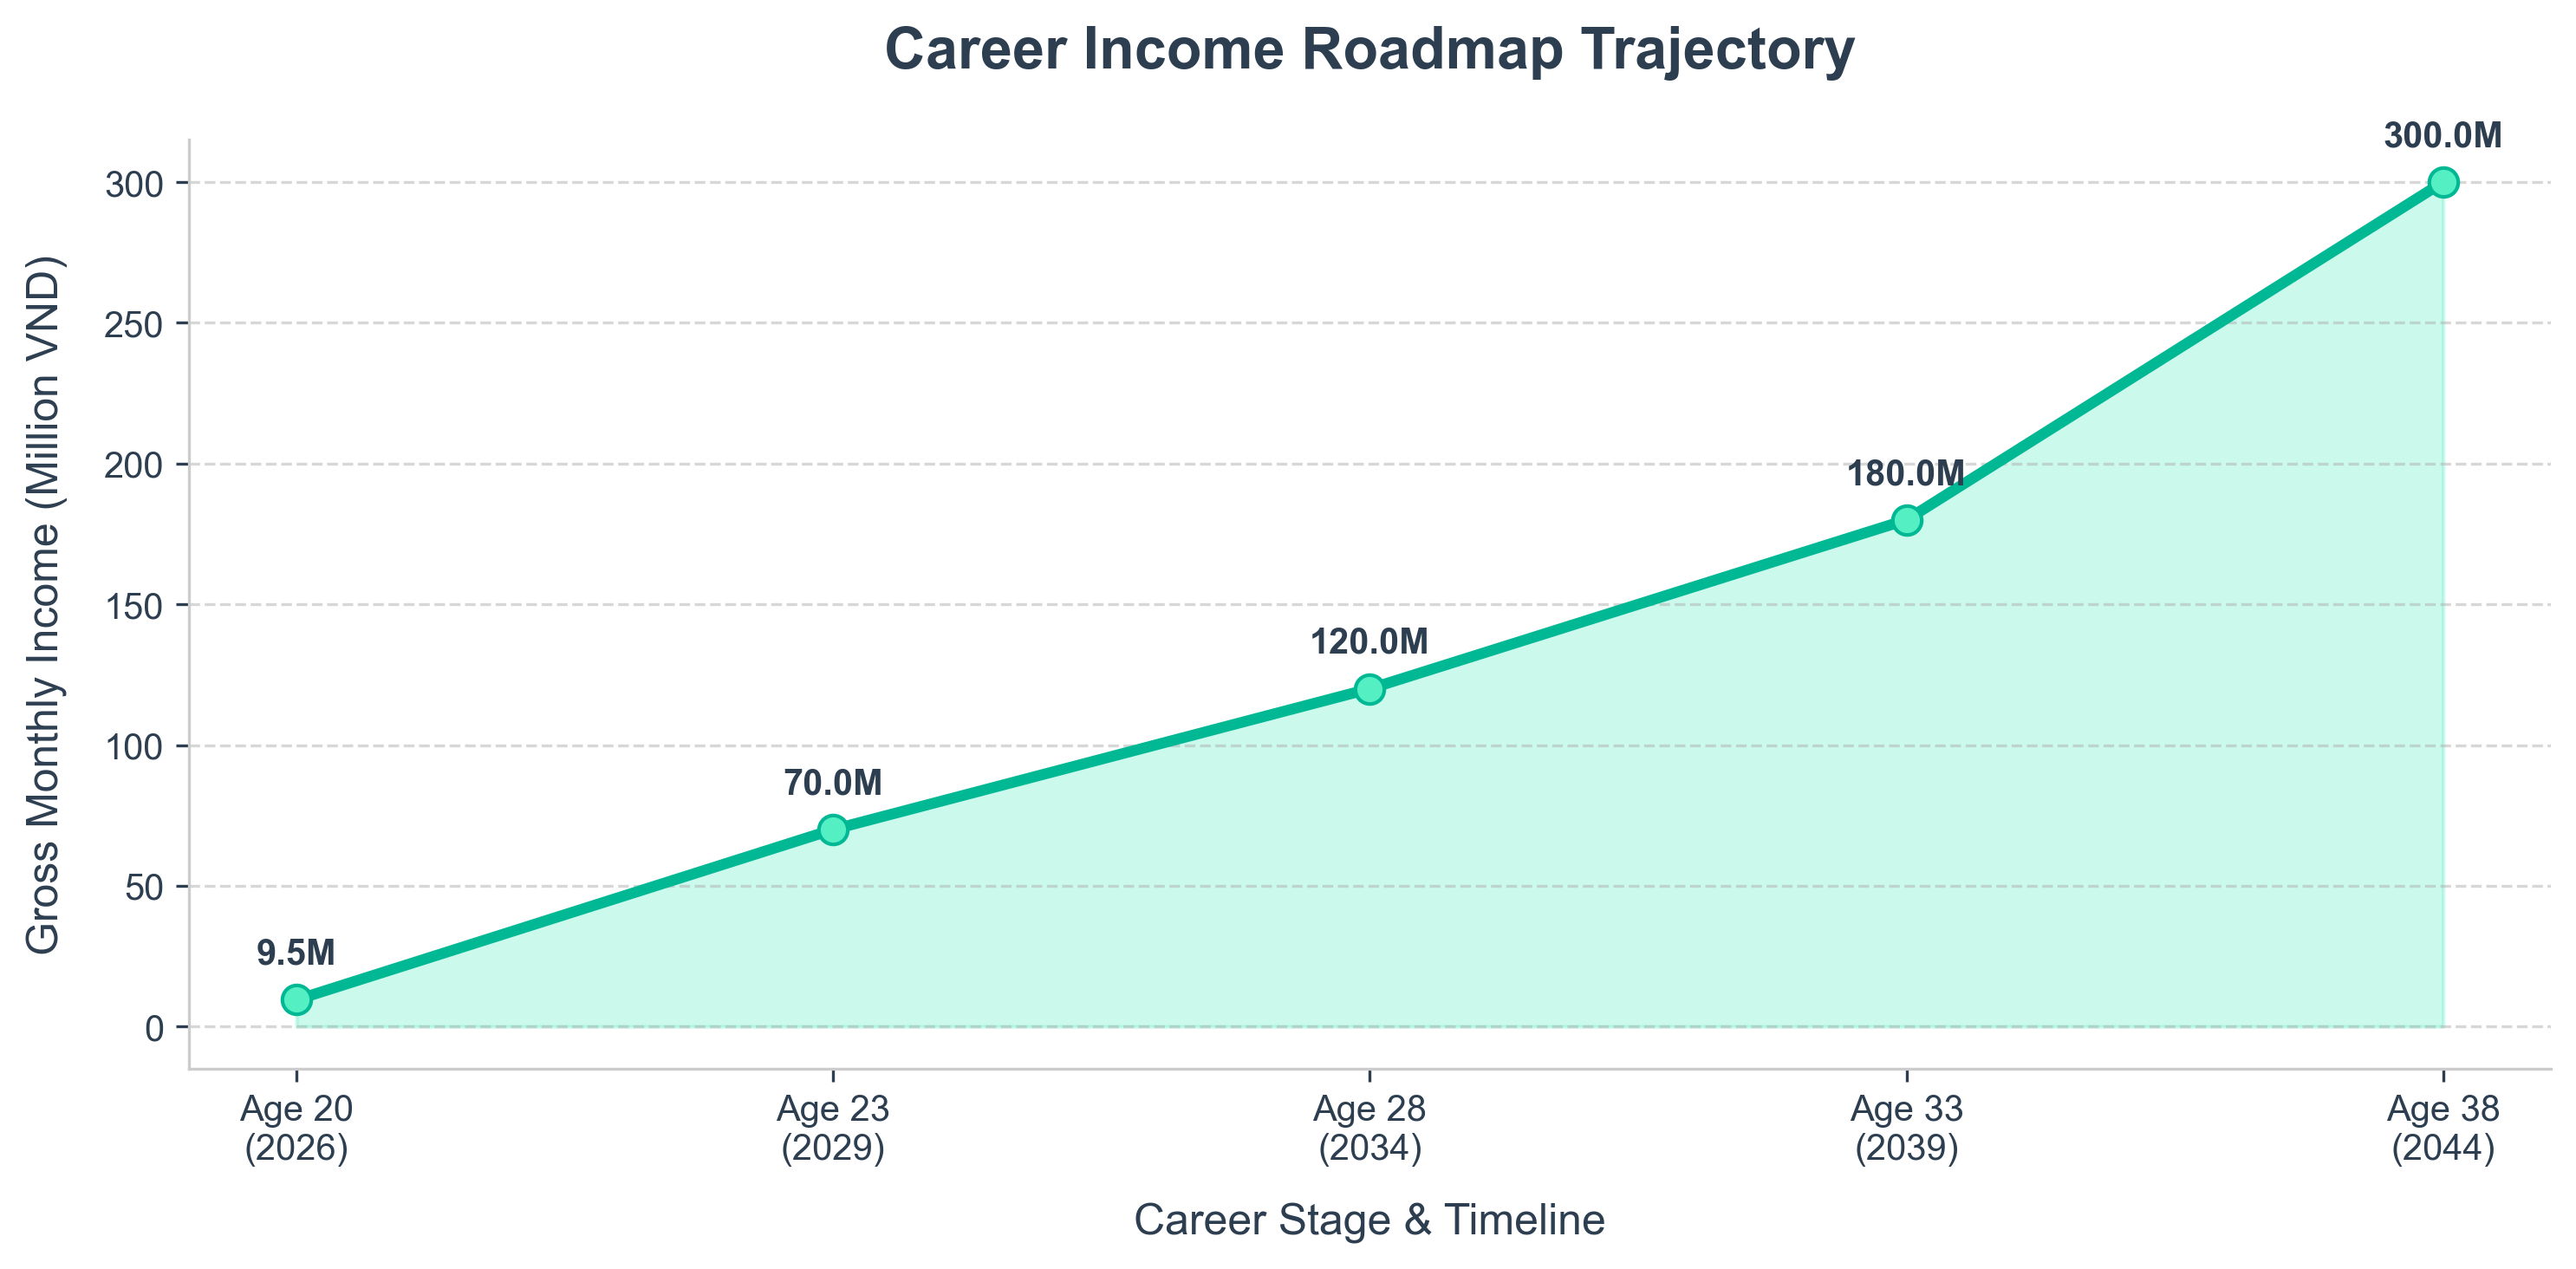
\includegraphics[width=\linewidth]{figures/income_trajectory.png}
  \caption{Career income roadmap from age 20 to 38}
  \label{fig:income_trajectory}
\end{minipage}

\vfill
\begin{center}
  \small\itshape Writing by Latex
\end{center}



\end{document}
